\documentclass[margin=3mm]{standalone}
\usepackage{tikz}
\usetikzlibrary{shapes, arrows}

\tikzstyle{startstop} = [rectangle, rounded corners, minimum width=2cm, minimum height=1cm, text centered, draw=black, text=white, fill=black!80]
\tikzstyle{statement} = [rectangle, minimum width=4cm, minimum height=1cm, text centered, draw=black, fill=blue!20]
\tikzstyle{decision} = [rectangle, minimum height=1cm, text centered, draw=black, fill=yellow!30]
\tikzstyle{edge} = [thick, ->, >=stealth]

\begin{document}
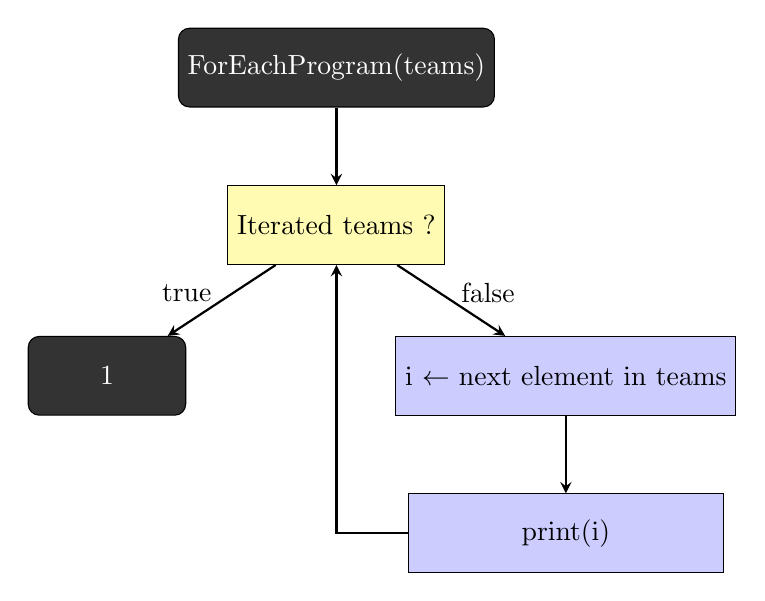
\begin{tikzpicture}[node distance=2cm]

\node (0) [startstop] {ForEachProgram(teams)};
\node (1) [decision, below of=0] {Iterated teams ?};
\node (2) [statement, yshift=-0.5cm, xshift=1.5cm, below right of=1] {i $\gets$ next element in teams};
\node (3) [statement, below of=2] {print(i)};
\node (4) [startstop, yshift=-0.5cm, xshift=-1.5cm, below left of=1] {1};

\draw [edge] (0) -- (1);
\draw [edge] (1) -- node[anchor=east, yshift=0.1cm]{true} (4);
\draw [edge] (1) -- node[anchor=west, yshift=0.1cm]{false} (2);
\draw [edge] (2) -- (3);
\draw [edge] (3) -| (1);

\end{tikzpicture}
\end{document}